
\chapter{Fundamentação} \label{ch:fundamentation}

Este Capítulo apresenta a fundamentação necessária para o entendimento do 
trabalho. Ele é separado em duas Seções, na primeira, são apresentadas as 
ferramentas de análise de desempenho de aplicações paralelas e, na segunda,
contextualizam-se plataformas e \emph{frameworks} utilizados no trabalho.

\section{Análise de desempenho de aplicações paralelas}

Para melhor organização do trabalho, esta Seção foi dividida em duas partes. A 
primeira apresenta ferramentas que oferecem visualização de rastros de 
aplicações desenvolvidas no modelo \emph{Bulk-synchronous parallel} (BSP), a 
segunda, contextualiza ferramentas voltadas para visualização de rastros de 
aplicações desenvolvidas no modelo orientado a tarefas.

\subsection{Ferramentas de visualização clássicas}

Essas ferramentas possuem o objetivo de prover visualizações de rastros para 
aplicações de HPC tradicionais. Estas eram desenvolvidas seguindo o modelo 
\emph{Bulk-Synchronous Parallel} (BSP), que consiste em uma série de 
\emph{supersteps} (computações, comunicações, sincronizações), executadas sobre 
um ambiente homogêneo. Como esta abordagem  dominou o cenário HPC durante muito 
tempo, suas necessidades balizaram o desenvolvimento da maior parte das 
ferramentas de análise de desempenho.

\subsubsection{ViTE}
ViTE \cite{ref:vite} é uma ferramenta de visualização de \emph{traces} 
open-source. Para o processamento de grandes entradas ele conta com aceleração 
de Hardware e OpenGL. Suas entradas são arquivos na linguagem Pajé 
\cite{ref:paje}.

Essa ferramenta exibe os recursos de forma hierárquica, onde oferece a 
visualização das tarefas (eixo vertical) em função de tempo (eixo horizontal), 
similar a um Gantt. Na análise de aplicações distribuídas, também é possível 
incluir indicadores de transferências de dados.

\subsubsection{Paraver}
Paraver \cite{ref:paraver} também objetiva a visualização e análise de 
\emph{traces} de execução. Ele conta com uma agregação de dados, definida pelo
usuário via arquivo de configuração, para conseguir exibir entradas volumosas. 
Suas entradas são geradas por vários modelos de programação, pela ferramenta 
Extrae.

\subsubsection{Vampir}
Vampir \cite{ref:vampir} é uma ferramenta proprietária de código fechado para 
fins de análise de \emph{traces}. Ela traz uma abordagem de cliente-servidor, 
onde o servidor pode ser executado no hardware de experimentação e o cliente é o 
computador do usuário.

Suas entradas são arquivos OTF2 (Open Trace Format, version 2) \cite{ref:otf2}.  
Ele fornece múltiplas visualizações como gráficos de espaço-tempo e estatísticas 
de execução.

\subsubsection{Ravel}
O objetivo da ferramenta Ravel \cite{ref:ravel} também é a visualização de 
\emph{traces}. Suas entradas são em formato OTF (\emph{Open Trace Format}) e 
sua diferença em relação aos demais é que ele mostra as linhas de tempo 
lógicas, fornecendo uma estruturação para melhor entendimento de operações.

\subsubsection{FrameSoc e Ocelotl}

FrameSoc \cite{ref:framesoc} é uma ferramenta de análise de performance, capaz 
de lidar com grandes volumes de dados. Como entrada, ela suporta diversos
formatos como Pajé, CTF, Paraver e OTF2. Além dos dados de \emph{trace}, é 
possível armazenar informações como metadados e anotações. A ferramenta converte 
tudo para um modelo de dados genérico e armazena em uma base de dados 
relacional.

Para visualizar grandes volumes de dados, a ferramenta baseia-se no Ocelotl 
\cite{ref:ocelotl}. Esse módulo possui um arquivo de configuração parametrizável 
pelo usuário, que gerencia uma agregação espaçotemporal dados.

\subsection{Ferramentas de visualização orientadas a tarefas}

Este modelo possui custo de execução de tarefas inconstante e costuma ser 
executado sobre um ambiente heterogêneo. Os analistas de desempenho que 
trabalham sobre as aplicações nesse cenário são diferentes, no modelo 
BSP é quem desenvolve a aplicação, neste é quem desenvolve o runtime. 

Devido a dominância do modelo BSP, a maior parte das ferramentas de 
visualização para o modelo corrente carrega características daquelas 
desenvolvidas para o predecessor. Todavia, as necessidades para análise de 
desempenho são diferentes tendo em vista que há diferenças impactantes entre 
ambos os modelos.


\subsubsection{DAGViz}

DAGViz \cite{ref:dagviz} é composto por dois passos: 

\begin{enumerate}
    \item extração do DAG dos arquivos de uma execução paralela;
    \item visualização hierárquica do DAG.
\end{enumerate}

Essa ferramenta traz uma visualização diferente do modelo BSP, exibindo as 
tarefas como um grafo hierárquico. Nele, o analista pode colapsar e expandir os 
grupos de tarefas. Dados de tempo de execução não são tratados pela ferramenta.

\subsubsection{Traces de execução com dependências de tarefas}

A ferramenta desenvolvida por \citet{ref:visuexecdep} traz um gráfico no estilo 
espaço-tempo (Gantt). Há algumas outras funcionalidades como a identificação de 
dependências de tarefas (apenas o primeiro nível) a medida que o usuário passa o 
mouse sobre as caixas que representam as tarefas.

Como entradas, são utilizados a representação do DAG e os \emph{traces} de 
execução. Essa ferramenta é desenvolvida especificamente para o 
\emph{runtime} PaRSEC.

\subsubsection{Temanejo}

Temanejo \cite{ref:temanejo} é um \emph{debugger} para o modelo de programação 
baseado em tarefas, onde o analista visualiza um DAG. Ele suporta grande parte 
dos \emph{runtimes} de execução de aplicações baseadas em tarefas, como OmpSs, 
StarPU e PaRSEC. Suas funcionalidades são focadas em depuração, permitindo que o 
usuário possa identificar e consertar parâmetros e dependências de tarefas.

\subsubsection{Delay Spotter}

Delay Spotter \cite{ref:delayspotter} é uma ferramenta, construída sobre o 
DAGViz, que possibilita a identificação de atrasos em \emph{runtimes}. Ela 
divide os estados dos \emph{workers} em três categorias, permitindo a 
identificação de delays decorrentes de problemas de escalonamento. Como em 
ambientes heterogêneos com tarefas variadas, a presença de \emph{delays} faz 
parte da execução das aplicações, essa ferramenta é pouco efetiva.

\subsubsection{TaskInsight}

TaskInsight \cite{ref:taskinsight} é uma ferramenta que objetiva identificar o 
comportamento de memória e seu impacto na execução de tarefas. Apesar de prover 
algumas estatísticas e possibilitar algumas identificações de anomalias, apenas 
essa análise não é o suficiente para identificar a maioria dos pontos de 
otimização de aplicações \emph{task-based}.

\subsubsection{StarVZ}

\emph{Framework} que é objeto deste trabalho, o StarVZ \cite{ref:starvz} possui 
a visualização de dados mais avançada dentre as ferramentas citadas. Construído 
com uma abordagem de \emph{script}, ela possui um grande poder de customização 
e, por isso, é difícil enumerar o que a ferramenta fornece. Ele será detalhado 
no Capítulo \ref{ch:starvz}.

\section{Ferramental para Big Data}

Esta Seção contextualiza o que será utilizado de ferramentas para 
tratamento de grandes volumes de dados que serão utilizadas neste trabalho. Na 
Seção \ref{ref:hadoop} contextualizamos a plataforma Hadoop e na Seção 
\ref{ref:spark} falamos sobre Spark.

\subsection{Hadoop} \label{ref:hadoop}


\begin{figure}[H]
 \centerline{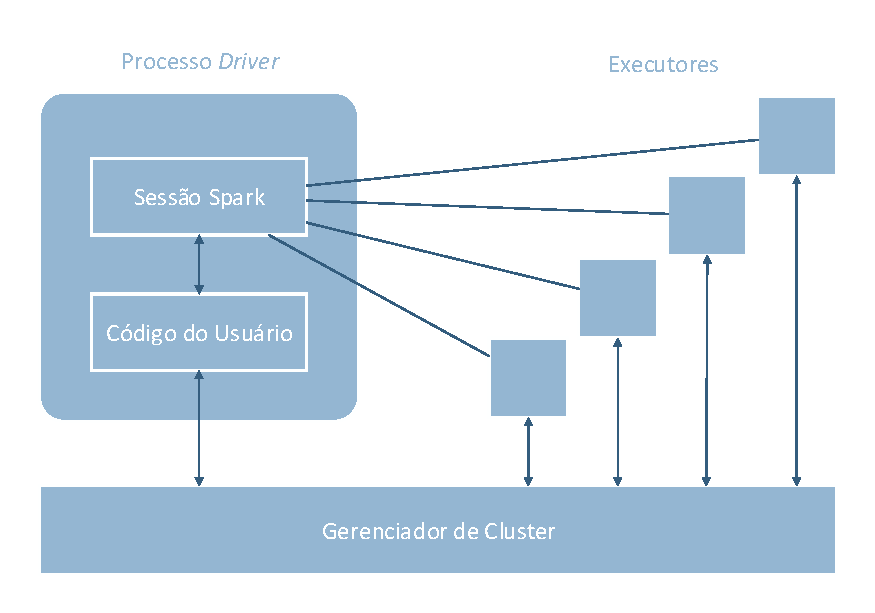
\includegraphics[width=1\textwidth]{./img/spark-arch.pdf}}
 \caption{Arquitetura de uma aplicação Spark.}
 \label{fig:spark-arch}
\end{figure}

O Hadoop é uma plataforma de código aberto que implementa o modelo de 
programação paralela MapReduce, desenvolvido pelo Google com o objetivo de 
processar grandes volumes de dados. Tal modelo baseia-se em duas primitivas 
presentes em linguagens funcionais: \emph{map} e \emph{reduce}. Esta abordagem 
foi adotada pois observaram que frequentemente era necessário mapear fragmentos 
de dados de uma entrada à uma chave identificadora e, em seguida, realizar 
computações sobre os dados mapeados para uma chave em comum 
\cite{ref:mapreduce}.

A Figura \ref{fig:mrworkflow} mostra o fluxo de execução básico do MapReduce. 
A Fase de \emph{Shuffle \& Merge} não será detalhada no trabalho, mas é 
importante salientar que existe um processamento entre as fases de mapeamento e 
redução.

\begin{figure}[ht]
 \centerline{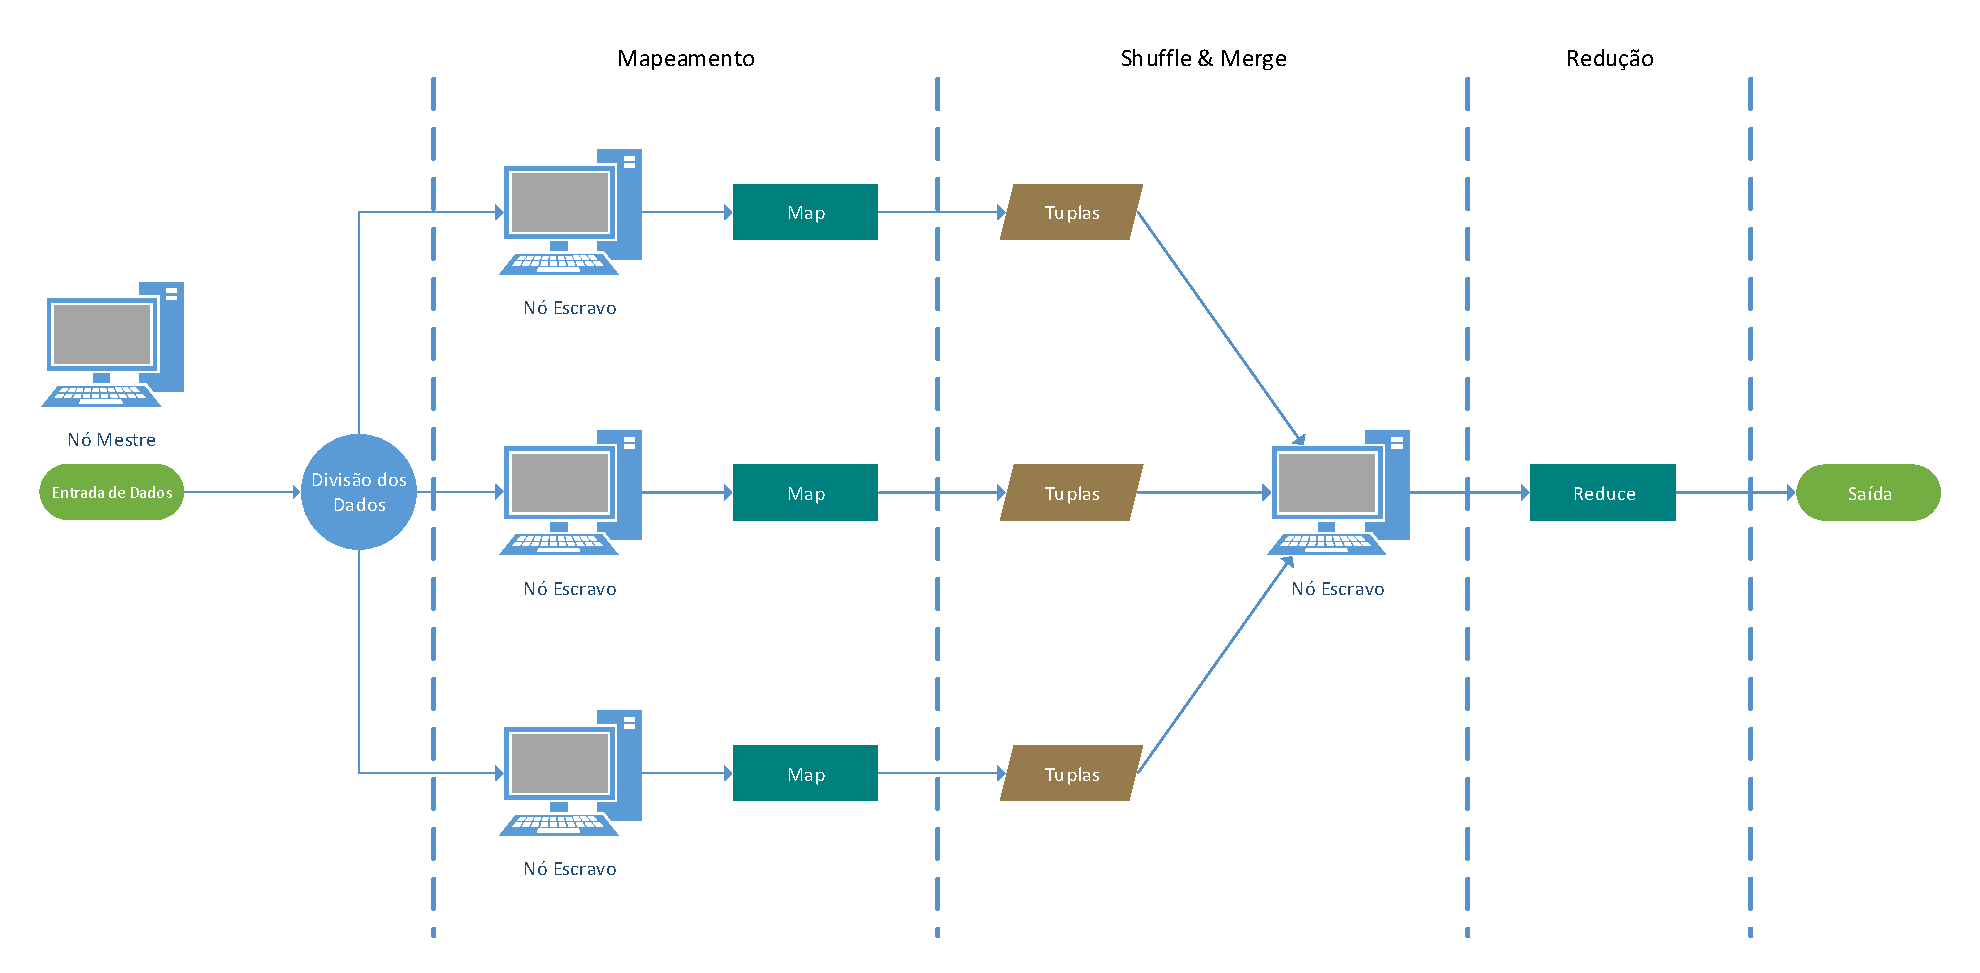
\includegraphics[width=1\textwidth]{./img/mapreduce-workflow.pdf}}
 \caption{\emph{Workflow} do MapReduce.}
 \label{fig:mrworkflow}
\end{figure}

Primeiramente temos os dados sendo inseridos no Sistema de Arquivos Distribuído 
\footnote{Termo em português para \emph{Distributed File System} (DFS). No caso 
do utilizado no Hadoop, tal sistema é referênciado como \emph{Hadoop Distributed 
File System} (HDFS).} da plataforma. Os arquivos são divididos em pedaços de 
tamanho fixo e armazenados sobre os nós da plataforma. Isso permite que os dados 
sejam tratados de forma rápida pois há paralelização em sua leitura.

Com os dados armazenados, pode se iniciar a fase de mapeamento, que resulta em 
conjuntos de tuplas intermediárias. Estas sofrem um pré-processamento na fase 
de \emph{Shuffle} e são disponibilizados para os nós que irão executar a fase 
de redução. Finalmente, os executores da redução obtém os dados e executam suas 
tarefas, gerando a saída da execução.

\subsection{Spark} \label{ref:spark}

Spark é um conjunto de uma engine unificada e um conjunto de bibliotecas para 
processamento de dados distribuídos \cite{ref:sparkbook}. A motivação para sua 
criação foi a necessidade de muitos tipos de processamento e a tendência das 
engines serem cada vez mais específicas no cenário de Big Data.

\begin{figure}[H]
 \centerline{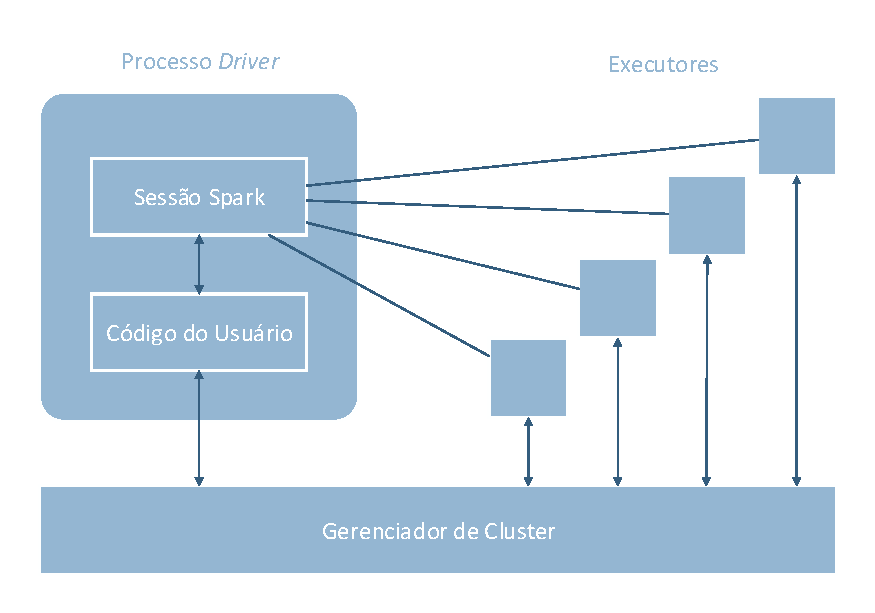
\includegraphics[width=1\textwidth]{./img/spark-arch.pdf}}
 \caption{Arquitetura de uma aplicação Spark.}
 \label{fig:spark-arch}
\end{figure}

A arquitetura do Spark pode ser visualizada na Figura \ref{fig:spark-arch}. A 
engine usualmente é executada sobre um cluster de máquinas gerenciado por um 
\texttt{Gerenciador de Cluster}, que mantém o controle dos recursos 
disponíveis. Ele oferece suporte a três gerenciadores: um próprio da engine, 
Hadoop YARN ou Mesos \cite{ref:mesos}.


O \texttt{driver process} é responsável por manter o ciclo de vida da 
aplicação. Dentre suas responsabilidades estão: responder às entradas do 
programa do usuário; analizar, distribuir e agendar trabalho sobre os 
\texttt{Executors}; e manter informação relevante sobre a execução. Os 
\texttt{executors} realizam duas funções: executam tarefas que lhes são 
atribuídas e reportam o estado das computações para o \texttt{driver process}.

O Spark é atrelado a um modelo de programação similar ao MapReduce, todavia, 
possui uma abstração para compartilhamento de dados, chamada \emph{Resilient 
Distributed Datasets} (RDDs). Estas, consistem em coleções de objetos tolerantes 
a falhas e que podem ser manipulados em paralelo e são particionados sobre a 
infraestrutura que executa a engine. 

Spark manipula RDDs através de uma API unificada disponibilizada para diversas 
linguagens, que facilita o desenvolvimento de aplicações. Nela, o usuário é 
capaz de passar funções locais para serem executadas de forma distribuída. A 
avaliação dos RDDs é realizada de forma \emph{Lazy}, o que significa que as 
manipulações são efetivadas apenas quando é executada uma ação no data frame. 
Isso permite que ele encontre um plano de execução eficiente pois pode agregar 
operações, otimizando o tempo de execução.





